%======================================================================
% University of Waterloo Thesis Template for LaTeX 
% Last Updated August 21, 2018 
% by Stephen Carr, IST Client Services, 
% University of Waterloo, 200 University Ave. W., Waterloo, Ontario, Canada
% FOR ASSISTANCE, please send mail to rt-IST-CSmathsci@rt.uwaterloo.ca

% DISCLAIMER
% To the best of our knowledge, this template satisfies the current uWaterloo thesis requirements.
% However, it is your responsibility to assure that you have met all 
% requirements of the University and your particular department.

% Many thanks for the feedback from many graduates who assisted the development of this template.
% Also note that there are explanatory comments and tips throughout this template.
%======================================================================
% Some important notes on using this template and making it your own...

% The University of Waterloo has required electronic thesis submission since October 2006. 
% See the uWaterloo thesis regulations at
% https://uwaterloo.ca/graduate-studies/thesis.
% This thesis template is geared towards generating a PDF 
% version optimized for viewing on an electronic display, including 
% hyperlinks within the PDF.

% DON'T FORGET TO ADD YOUR OWN NAME AND TITLE in the "hyperref" package
% configuration below. THIS INFORMATION GETS EMBEDDED IN THE PDF FINAL PDF DOCUMENT.
% You can view the information if you view properties of the PDF document.

% Many faculties/departments also require one or more printed
% copies. This template attempts to satisfy both types of output. See additional notes below.
% It is based on the standard "book" document class which provides all necessary 
% sectioning structures and allows multi-part theses.

% If you are using this template in Overleaf (cloud-based collaboration service), then it is 
% automatically processed and previewed for you as you edit.

% For people who prefer to install their own LaTeX distributions on their own computers, and process 
% the source files manually, the following notes provide the sequence of tasks:
 
% E.g. to process a thesis called "mythesis.tex" based on this template, run:

% pdflatex mythesis	-- first pass of the pdflatex processor
% bibtex mythesis	-- generates bibliography from .bib data file(s)
% makeindex         -- should be run only if an index is used 
% pdflatex mythesis	-- fixes numbering in cross-references, bibliographic references, glossaries, index, etc.
% pdflatex mythesis	-- it takes a couple of passes to completely process all cross-references

% If you use the recommended LaTeX editor, Texmaker, you would open the mythesis.tex
% file, then click the PDFLaTeX button. Then run BibTeX (under the Tools menu).
% Then click the PDFLaTeX button two more times. If you have an index as well,
% you'll need to run MakeIndex from the Tools menu as well, before running pdflatex
% the last two times.

% N.B. The "pdftex" program allows graphics in the following formats to be
% included with the "\includegraphics" command: PNG, PDF, JPEG, TIFF
% Tip 1: Generate your figures and photos in the size you want them to appear
% in your thesis, rather than scaling them with \includegraphics options.
% Tip 2: Any drawings you do should be in scalable vector graphic formats:
% SVG, PNG, WMF, EPS and then converted to PNG or PDF, so they are scalable in
% the final PDF as well.
% Tip 3: Photographs should be cropped and compressed so as not to be too large.

% To create a PDF output that is optimized for double-sided printing: 
%
% 1) comment-out the \documentclass statement in the preamble below, and
% un-comment the second \documentclass line.
%
% 2) change the value assigned below to the boolean variable
% "PrintVersion" from "false" to "true".

%======================================================================
%   D O C U M E N T   P R E A M B L E
% Specify the document class, default style attributes, and page dimensions, etc.
% For hyperlinked PDF, suitable for viewing on a computer, use this:
\documentclass[letterpaper,12pt,titlepage,oneside,final]{book}
 
% For PDF, suitable for double-sided printing, change the PrintVersion variable below
% to "true" and use this \documentclass line instead of the one above:
%\documentclass[letterpaper,12pt,titlepage,openright,twoside,final]{book}

% Some LaTeX commands I define for my own nomenclature.
% If you have to, it's easier to make changes to nomenclature once here than in a 
% million places throughout your thesis!
\newcommand{\package}[1]{\textbf{#1}} % package names in bold text
\newcommand{\cmmd}[1]{\textbackslash\texttt{#1}} % command name in tt font 
\newcommand{\href}[1]{#1} % does nothing, but defines the command so the
    % print-optimized version will ignore \href tags (redefined by hyperref pkg).
%\newcommand{\texorpdfstring}[2]{#1} % does nothing, but defines the command
% Anything defined here may be redefined by packages added below...

% This package allows if-then-else control structures.
\usepackage{ifthen}
\newboolean{PrintVersion}
\setboolean{PrintVersion}{false}
% CHANGE THIS VALUE TO "true" as necessary, to improve printed results for hard copies
% by overriding some options of the hyperref package, called below.

%\usepackage{nomencl} % For a nomenclature (optional; available from ctan.org)
\usepackage{amsmath,amssymb,amstext} % Lots of math symbols and environments
\usepackage[pdftex]{graphicx} % For including graphics N.B. pdftex graphics driver 

% Hyperlinks make it very easy to navigate an electronic document.
% In addition, this is where you should specify the thesis title
% and author as they appear in the properties of the PDF document.
% Use the "hyperref" package 
% N.B. HYPERREF MUST BE THE LAST PACKAGE LOADED; ADD ADDITIONAL PKGS ABOVE
\usepackage[pdftex,pagebackref=false]{hyperref} % with basic options
%\usepackage[pdftex,pagebackref=true]{hyperref}
		% N.B. pagebackref=true provides links back from the References to the body text. This can cause trouble for printing.
\hypersetup{
    plainpages=false,       % needed if Roman numbers in frontpages
    unicode=false,          % non-Latin characters in Acrobat’s bookmarks
    pdftoolbar=true,        % show Acrobat’s toolbar?
    pdfmenubar=true,        % show Acrobat’s menu?
    pdffitwindow=false,     % window fit to page when opened
    pdfstartview={FitH},    % fits the width of the page to the window
%    pdftitle={uWaterloo\ LaTeX\ Thesis\ Template},    % title: CHANGE THIS TEXT!
    pdfauthor={Zeynep Akkalyoncu Yilmaz},    % author: CHANGE THIS TEXT! and uncomment this line
%    pdfsubject={Subject},  % subject: CHANGE THIS TEXT! and uncomment this line
%    pdfkeywords={keyword1} {key2} {key3}, % list of keywords, and uncomment this line if desired
    pdfnewwindow=true,      % links in new window
    colorlinks=true,        % false: boxed links; true: colored links
    linkcolor=blue,         % color of internal links
    citecolor=green,        % color of links to bibliography
    filecolor=magenta,      % color of file links
    urlcolor=cyan           % color of external links
}
\ifthenelse{\boolean{PrintVersion}}{   % for improved print quality, change some hyperref options
\hypersetup{	% override some previously defined hyperref options
%    colorlinks,%
    citecolor=black,%
    filecolor=black,%
    linkcolor=black,%
    urlcolor=black}
}{} % end of ifthenelse (no else)

\usepackage[automake,toc,abbreviations]{glossaries-extra} % Exception to the rule of hyperref being the last add-on package
% If glossaries-extra is not in your LaTeX distribution, get it from CTAN (http://ctan.org/pkg/glossaries-extra), 
% although it's supposed to be in both the TeX Live and MikTeX distributions. There are also documentation and 
% installation instructions there.

% Setting up the page margins...
% uWaterloo thesis requirements specify a minimum of 1 inch (72pt) margin at the
% top, bottom, and outside page edges and a 1.125 in. (81pt) gutter
% margin (on binding side). While this is not an issue for electronic
% viewing, a PDF may be printed, and so we have the same page layout for
% both printed and electronic versions, we leave the gutter margin in.
% Set margins to minimum permitted by uWaterloo thesis regulations:
\setlength{\marginparwidth}{0pt} % width of margin notes
% N.B. If margin notes are used, you must adjust \textwidth, \marginparwidth
% and \marginparsep so that the space left between the margin notes and page
% edge is less than 15 mm (0.6 in.)
\setlength{\marginparsep}{0pt} % width of space between body text and margin notes
\setlength{\evensidemargin}{0.125in} % Adds 1/8 in. to binding side of all 
% even-numbered pages when the "twoside" printing option is selected
\setlength{\oddsidemargin}{0.125in} % Adds 1/8 in. to the left of all pages
% when "oneside" printing is selected, and to the left of all odd-numbered
% pages when "twoside" printing is selected
\setlength{\textwidth}{6.375in} % assuming US letter paper (8.5 in. x 11 in.) and 
% side margins as above
\raggedbottom

% The following statement specifies the amount of space between
% paragraphs. Other reasonable specifications are \bigskipamount and \smallskipamount.
\setlength{\parskip}{\medskipamount}

% The following statement controls the line spacing.  The default
% spacing corresponds to good typographic conventions and only slight
% changes (e.g., perhaps "1.2"), if any, should be made.
\renewcommand{\baselinestretch}{1} % this is the default line space setting

% By default, each chapter will start on a recto (right-hand side)
% page.  We also force each section of the front pages to start on 
% a recto page by inserting \cleardoublepage commands.
% In many cases, this will require that the verso (left-hand) page be
% blank, and while it should be counted, a page number should not be
% printed.  The following statements ensure a page number is not
% printed on an otherwise blank verso page.
\let\origdoublepage\cleardoublepage
\newcommand{\clearemptydoublepage}{%
  \clearpage{\pagestyle{empty}\origdoublepage}}
\let\cleardoublepage\clearemptydoublepage

% Define Glossary terms (This is properly done here, in the preamble and could also be \input{} from a separate file...)
% Main glossary entries -- definitions of relevant terminology
\newglossaryentry{computer}
{
name=computer,
description={A programmable machine that receives input data,
               stores and manipulates the data, and provides
               formatted output}
}

% Nomenclature glossary entries -- New definitions, or unusual terminology
\newglossary*{nomenclature}{Nomenclature}
\newglossaryentry{dingledorf}
{
type=nomenclature,
name=dingledorf,
description={A person of supposed average intelligence who makes incredibly brainless misjudgments}
}

% List of Abbreviations (abbreviations type is built in to the glossaries-extra package)
\newabbreviation{aaaaz}{AAAAZ}{American Association of Amateur Astronomers and Zoologists}

% List of Symbols
\newglossary*{symbols}{List of Symbols}
\newglossaryentry{rvec}
{
name={$\mathbf{v}$},
sort={label},
type=symbols,
description={Random vector: a location in n-dimensional Cartesian space, where each dimensional component is determined by a random process}
}
 
\makeglossaries

%%% 
\newcommand\myworries[1]{\textcolor{red}{#1}}

\usepackage{framed}
\usepackage{booktabs}
\usepackage{rotating}

%======================================================================
%   L O G I C A L    D O C U M E N T
% The logical document contains the main content of your thesis.
% Being a large document, it is a good idea to divide your thesis
% into several files, each one containing one chapter or other significant 
% chunk of content, so you can easily shuffle things around later if desired.
%======================================================================
\begin{document}

%----------------------------------------------------------------------
% FRONT MATERIAL
% title page,declaration, borrowers' page, abstract, acknowledgements,
% dedication, table of contents, list of tables, list of figures, nomenclature, etc.
%----------------------------------------------------------------------
% T I T L E   P A G E
% -------------------
% Last updated June 14, 2017, by Stephen Carr, IST-Client Services
% The title page is counted as page `i' but we need to suppress the
% page number. Also, we don't want any headers or footers.
\pagestyle{empty}
\pagenumbering{roman}

% The contents of the title page are specified in the "titlepage"
% environment.
\begin{titlepage}
        \begin{center}
        \vspace*{1.0cm}

        \Huge
        {\bf University of Waterloo E-Thesis Template for \LaTeX }

        \vspace*{1.0cm}

        \normalsize
        by \\

        \vspace*{1.0cm}

        \Large
        Zeynep Akkalyoncu Yilmaz \\

        \vspace*{3.0cm}

        \normalsize
        A thesis \\
        presented to the University of Waterloo \\ 
        in fulfillment of the \\
        thesis requirement for the degree of \\
        Master of Mathematics \\
        in \\
        Computer Science \\

        \vspace*{2.0cm}

        Waterloo, Ontario, Canada, 2019 \\

        \vspace*{1.0cm}

        \copyright\ Zeynep Akkalyoncu Yilmaz 2019 \\
        \end{center}
\end{titlepage}

% The rest of the front pages should contain no headers and be numbered using Roman numerals starting with `ii'
\pagestyle{plain}
\setcounter{page}{2}

\cleardoublepage % Ends the current page and causes all figures and tables that have so far appeared in the input to be printed.
% In a two-sided printing style, it also makes the next page a right-hand (odd-numbered) page, producing a blank page if necessary.

 
% E X A M I N I N G   C O M M I T T E E (Required for Ph.D. theses only)
% Remove or comment out the lines below to remove this page
%\begin{center}\textbf{Examining Committee Membership}\end{center}
%  \noindent
%The following served on the Examining Committee for this thesis. The decision of the Examining Committee is by majority vote.
%  \bigskip
%  
%  \noindent
%\begin{tabbing}
%Internal-External Member: \=  \kill % using longest text to define tab length
%External Examiner: \>  Bruce Bruce \\ 
%\> Professor, Dept. of Philosophy of Zoology, University of Wallamaloo \\
%\end{tabbing} 
%  \bigskip
%  
%  \noindent
%\begin{tabbing}
%Internal-External Member: \=  \kill % using longest text to define tab length
%Supervisor(s): \> Doris Johnson \\
%\> Professor, Dept. of Zoology, University of Waterloo \\
%\> Andrea Anaconda \\
%\> Professor Emeritus, Dept. of Zoology, University of Waterloo \\
%\end{tabbing}
%  \bigskip
%  
%  \noindent
%  \begin{tabbing}
%Internal-External Member: \=  \kill % using longest text to define tab length
%Internal Member: \> Pamela Python \\
%\> Professor, Dept. of Zoology, University of Waterloo \\
%\end{tabbing}
%  \bigskip
%  
%  \noindent
%\begin{tabbing}
%Internal-External Member: \=  \kill % using longest text to define tab length
%Internal-External Member: \> Deepa Thotta \\
%\> Professor, Dept. of Philosophy, University of Waterloo \\
%\end{tabbing}
%  \bigskip
%  
%  \noindent
%\begin{tabbing}
%Internal-External Member: \=  \kill % using longest text to define tab length
%Other Member(s): \> Leeping Fang \\
%\> Professor, Dept. of Fine Art, University of Waterloo \\
%\end{tabbing}

\cleardoublepage

% D E C L A R A T I O N   P A G E
% -------------------------------
  % The following is a sample Delaration Page as provided by the GSO
  % December 13th, 2006.  It is designed for an electronic thesis.
%  \noindent
%I hereby declare that I am the sole author of this thesis. This is a true copy of the thesis, including any required final revisions, as accepted by my examiners.
%
%  \bigskip
%  
%  \noindent
%I understand that my thesis may be made electronically available to the public.

\cleardoublepage

% A B S T R A C T
% ---------------

\begin{center}\textbf{Abstract}\end{center}
Standard bag-of-words term-matching techniques in document retrieval fail to exploit rich semantic information embedded in the document texts.
One promising recent trend in facilitating context-aware semantic matching has been the development of massively pretrained language models, culminating in BERT as its most popular example today.
In this work, we propose adapting BERT as a neural reranker for document retrieval with large improvements on news articles.
Two fundamental issues arise in applying BERT to ``ad hoc'' document retrieval on newswire collections:\
relevance judgements in existing test collections are provided only at the document level, and documents often exceed the length that BERT was designed to handle.
To overcome these challenges, we compute and aggregate sentence-level relevance scores to rank documents.
We solve the problem of lack of appropriate relevance judgements by leveraging sentence-level and passage-level relevance judgements available in collections from other domains to capture cross-domain notions of relevance.
We demonstrate that models of relevance can be transferred across domains.
By leveraging semantic cues learned across various domains, we propose a model that achieves state-of-the-art results across three standard TREC newswire collections.
We explore the effects of cross-domain relevance transfer, and trade-offs between using document and sentence scores for document ranking.
We also present an end-to-end document retrieval system that incorporates the open-source Anserini information retrieval toolkit, discussing the related technical challenges and design decisions.

\cleardoublepage

% A C K N O W L E D G E M E N T S
% -------------------------------

\begin{center}\textbf{Acknowledgements}\end{center}

I would like to thank all the little people who made this thesis possible.
\cleardoublepage

% D E D I C A T I O N
% -------------------

\begin{center}\textbf{Dedication}\end{center}

This is dedicated to the one I love.
\cleardoublepage

% T A B L E   O F   C O N T E N T S
% ---------------------------------
\renewcommand\contentsname{Table of Contents}
\tableofcontents
\cleardoublepage
\phantomsection    % allows hyperref to link to the correct page

% L I S T   O F   T A B L E S
% ---------------------------
\addcontentsline{toc}{chapter}{List of Tables}
\listoftables
\cleardoublepage
\phantomsection		% allows hyperref to link to the correct page

% L I S T   O F   F I G U R E S
% -----------------------------
\addcontentsline{toc}{chapter}{List of Figures}
\listoffigures
\cleardoublepage
\phantomsection		% allows hyperref to link to the correct page

% GLOSSARIES (Lists of definitions, abbreviations, symbols, etc. provided by the glossaries-extra package)
% -----------------------------
\printglossaries
\cleardoublepage
\phantomsection		% allows hyperref to link to the correct page

% Change page numbering back to Arabic numerals
\pagenumbering{arabic}

 

%----------------------------------------------------------------------
% MAIN BODY
% We suggest using a separate file for each chapter of your thesis.
% Start each chapter file with the \chapter command.
% Only use \documentclass or \begin{document} and \end{document} commands 
% in this master document.
% Tip 4: Putting each sentence on a new line is a way to simplify later editing.
%----------------------------------------------------------------------
%======================================================================
\chapter{Introduction}
%======================================================================

Document retrieval refers to the task of generating a ranking of documents from a large corpus $ D $ in response to a query $ Q $.
In a typical document retrieval pipeline, an inverted index is constructed in advance from the collection, which often comprises unstructured text documents, for fast access during retrieval.
When the user issues a query, the query representation is matched against the index, computing a similarity score for each document.
The top most relevant documents based on their closeness to the query are returned to the user in order of relevance.
This procedure may be followed by a subsequent re-ranking stage where the candidate documents outputted by the previous step are further re-ranked in a way that maximizes some retrieval metric such as average precision (AP).

\begin{figure}[b!]
	\begin{framed}
		\centering
    		\textbf{Query:} international art crime \\
    		\textbf{Text:} The thieves demand a ransom of \$2.2 million for the works and return one of them.
	\end{framed}
\label{query-sent-example}
 \caption{An example of a query-text pair from the TREC Robust04 collection where a relevant piece of text does not contain direct query matches.}
\end{figure}

Document retrieval systems traditionally rely on term-matching techniques, such as BM25, to judge the relevance of documents in a corpus.
More specifically, the more common terms a document shares with the query, the more relevant it is considered.
As a result, these systems may fail to detect documents that do not contain the exact query terms, but are nonetheless relevant.
For example, consider a document that expresses relevant information in a way that cannot be resolved without the use of external semantic tools.
Figure \ref{query-sent-example} displays one such query-text pair where words semantically close to the query need to be identified to establish relevance.
This ``vocabulary mismatch'' problem represents a long-standing challenge in information retrieval.
To put its significance into context, Zhao et al. \cite{zhao2010term} show that the average query terms may not appear in as many as 40\% of relevant documents in TREC ``ad hoc'' retrieval datasets.

Clearly, the classic exact matching approach to document retrieval neglects to exploit rich semantic information embedded in the documents.
To overcome this shortcoming, a number of models such as Latent Semantic Analysis \cite{deerwester1990indexing} that maps both queries and documents into distributed representations has been proposed.
This innovation has enabled semantic matching to aid in document retrieval by extracting useful semantic matching signals.
With the advent of neural networks, neural language models have been quickly adopted to learn better distributed representations of text.
\myworries{How much better? Why?}
Moreover, deep neural models have eliminated the need to manually engineer natural language features.
Therefore, deep neural networks have since largely replaced the earlier models based on manual decomposition of document matrices.
\myworries{Examples...}

%Despite growing interest in neural networks, some researchers have recently voiced concern as to whether their use has truly contributed to progress in the field of information retrieval \myworries{citation}.
%\myworries{Take stuff from their neural hype paper}

One recent innovation that has changed the tide in NLP research has been massively pre-trained language models with its most popular example today being Bidirectional Encoder Representation Transformers (BERT) \cite{devlin2018bert}.
BERT has achieved state-of-the-art results across a wide range of NLP tasks from question answering to machine translation.
While BERT has enjoyed widespread adoption across the NLP community, its application in information retrieval research has been limited in comparison.
Guo et al. \cite{guo2016deep} suggest that the lackluster success of deep neural networks in information retrieval may be owing to the fact that crucial characteristics of the ``ad hoc'' document retrieval task are not properly addressed.
Specifically, they emphasize that the relevance matching problem in information retrieval and semantic matching problem in natural language processing are fundamentally different in that the former depends heavily on exact matching signals, query term importance and diverse matching requirements.
In other words, it is crucial to strike a good balance between exact and semantic matching in document retrieval.
For this reason, neural models are usually involved in multi-stage architectures where a list of candidate documents are retrieved with a standard bag-of-words term-matching technique as described above.
The documents in this list are then rescored and reranked by the neural model.
\myworries{Some notable examples include...}

%%%

In this thesis, we present a novel way to apply BERT to ``ad hoc'' document retrieval on long documents -- particularly, newswire articles.
A BERT reranker is deployed as part of an end-to-end document retrieval pipeline with significant improvements on standard TREC newswire collections.
Specifically, we adapt BERT for binary relevance classification over text to capture notions of relevance.
\myworries{One more sentence to describe?}
We point out that applying BERT to document retrieval on newswire documents is not trivial due to two principal challenges.
Firist of all, BERT has a maximum input length of 512 tokens, which is insufficient to accommodate the entirety of most news articles.
To put this into perspective, a typical TREC Robust04 document has a median length of 679 tokens, and in fact, 66\% of all documents are longer than 512 tokens.
Secondly, most collections provide relevance judgements only at the document level.
Therefore, we only know what documents are relevant for a given query, but not the specific spans within the document.
To further aggravate this issue, a document is considered relevant as long as some part of it is relevant, and most of the document often has nothing to do with the query.

We address the abovementioned challenges by proposing two effective innovations:\
First, instead of relying solely on document-level relevance judgements, we aggregate sentence-level evidence to rank documents.
As mentioned before, since standard newswire collections lack sentence level judgements to facilitate this approach, we instead explore leveraging sentence-level or passage-level judgements already available in collections in other domains, such as tweets and reading comprehension.
To this end, we fine-tune BERT models on these collections to learn models of relevance.
Surprisingly, we demonstrate that models of relevance can indeed be successfully transferred across domains.
%We are able to use BERT models trained on out-of-domain collections on newswire documents to compute a relevance score for each constituent sentence.
It is important to note that the representational power of neural networks come at the cost of challenges in interpretability.
For this reason, we dedicate a portion of this thesis to error analysis experiments in an attempt to qualify and better understand the cross-domain transfer effects.
We also elaborate on the challenges encountered in the implementation of such an end-to-end retrieval pipeline in an attempt to bridge the worlds of natural language processing and information retrieval from a software engineering perspective.

\section{Contributions}

The main contributions of this thesis can be summarized as follows:\\

\begin{itemize}
\item
We present two innovations to successfully apply BERT to \textit{ad hoc} document retrieval with large improvements:\
integrating sentence-level evidence to address the fact that BERT cannot process long spans posed by newswire documents, and exploiting cross-domain models of relevance for collections without sentence- or passage-level annotations.
\item
We explore through various error analysis experiments on the effects of cross-domain relevance transfer with BERT as well as the contributions of BM25 and sentence scores to the final document ranking.
\item 
With the proposed model, we establish state-of-the-art effectiveness on three standard TREC newswire collections at the time of writing.\
\myworries{neural or otherwise}
\item
We release an end-to-end pipeline that applies BERT to document retrieval over large document collections via integration with the open-source Anserini information retrieval toolkit.
We elaborate on the technical challenges in the integration of NLP and IR capabilities, along with the design rationale behind our approach to tightly-coupled integration between Python to support neural networks and the Java Virtual Machine to support document retrieval using the open-source Lucene search library.
\myworries{something about demo, TREC DL...}

\end{itemize}

\section{Thesis Organization}

The remainder of this thesis is organized in the following order:\
\myworries{add link to actual chapters}
Chapter 2 reviews related work in neural document retrieval, particularly applications of BERT to document retrieval.
Chapter 3 motivates the approach with some background information on the task, and introduces the datasets used for both training and evaluation as well as metrics.
Chapter 4 proposes an end-to-end pipeline for document retrieval with BERT by elaborating on the design decisions and challenges.
\myworries{What about TREC DL? MS MARCO?}
Chapter 5 describes the experimental setup, and presents the results on three newswire collections -- Robust04, Core17 and Core18.
Chapter 6 concludes the thesis by summarizing the contributions and discussing future work.

%In the beginning, there was $\pi$:
%
%\begin{equation}
%   e^{\pi i} + 1 = 0  \label{eqn_pi}
%\end{equation}
%A \gls{computer} could compute $\pi$ all day long. In fact, subsets of digits of $\pi$'s decimal approximation would make a good source for psuedo-random vectors, \gls{rvec} . 
%
%%----------------------------------------------------------------------
%\section{State of the Art}
%%----------------------------------------------------------------------
%
%See equation \ref{eqn_pi} on page \pageref{eqn_pi}.\footnote{A famous equation.}
%
%\section{Some Meaningless Stuff}
%
%The credo of the \gls{aaaaz} was, for several years, several paragraphs of gibberish, until the \gls{dingledorf} responsible for the \gls{aaaaz} Web site realized his mistake:
%
%"Velit dolor illum facilisis zzril ipsum, augue odio, accumsan ea augue molestie lobortis zzril laoreet ex ad, adipiscing nulla. Veniam dolore, vel te in dolor te, feugait dolore ex vel erat duis nostrud diam commodo ad eu in consequat esse in ut wisi. Consectetuer dolore feugiat wisi eum dignissim tincidunt vel, nostrud, at vulputate eum euismod, diam minim eros consequat lorem aliquam et ad. Feugait illum sit suscipit ut, tation in dolore euismod et iusto nulla amet wisi odio quis nisl feugiat adipiscing luptatum minim nisl, quis, erat, dolore. Elit quis sit dolor veniam blandit ullamcorper ex, vero nonummy, duis exerci delenit ullamcorper at feugiat ullamcorper, ullamcorper elit vulputate iusto esse luptatum duis autem. Nulla nulla qui, te praesent et at nisl ut in consequat blandit vel augue ut.
%
%Illum suscipit delenit commodo augue exerci magna veniam hendrerit dignissim duis ut feugait amet dolor dolor suscipit iriure veniam. Vel quis enim vulputate nulla facilisis volutpat vel in, suscipit facilisis dolore ut veniam, duis facilisi wisi nulla aliquip vero praesent nibh molestie consectetuer nulla. Wisi nibh exerci hendrerit consequat, nostrud lobortis ut praesent dignissim tincidunt enim eum accumsan. Lorem, nonummy duis iriure autem feugait praesent, duis, accumsan tation enim facilisi qui te dolore magna velit, iusto esse eu, zzril. Feugiat enim zzril, te vel illum, lobortis ut tation, elit luptatum ipsum, aliquam dolor sed. Ex consectetuer aliquip in, tation delenit dignissim accumsan consequat, vero, et ad eu velit ut duis ea ea odio.
%
%Vero qui, te praesent et at nisl ut in consequat blandit vel augue ut dolor illum facilisis zzril ipsum. Exerci odio, accumsan ea augue molestie lobortis zzril laoreet ex ad, adipiscing nulla, et dolore, vel te in dolor te, feugait dolore ex vel erat duis. Ut diam commodo ad eu in consequat esse in ut wisi aliquip dolore feugiat wisi eum dignissim tincidunt vel, nostrud. Ut vulputate eum euismod, diam minim eros consequat lorem aliquam et ad luptatum illum sit suscipit ut, tation in dolore euismod et iusto nulla. Iusto wisi odio quis nisl feugiat adipiscing luptatum minim. Illum, quis, erat, dolore qui quis sit dolor veniam blandit ullamcorper ex, vero nonummy, duis exerci delenit ullamcorper at feugiat. Et, ullamcorper elit vulputate iusto esse luptatum duis autem esse nulla qui.
%
%Praesent dolore et, delenit, laoreet dolore sed eros hendrerit consequat lobortis. Dolor nulla suscipit delenit commodo augue exerci magna veniam hendrerit dignissim duis ut feugait amet. Ad dolor suscipit iriure veniam blandit quis enim vulputate nulla facilisis volutpat vel in. Erat facilisis dolore ut veniam, duis facilisi wisi nulla aliquip vero praesent nibh molestie consectetuer nulla, iriure nibh exerci hendrerit. Vel, nostrud lobortis ut praesent dignissim tincidunt enim eum accumsan ea, nonummy duis. Ad autem feugait praesent, duis, accumsan tation enim facilisi qui te dolore magna velit, iusto esse eu, zzril vel enim zzril, te. Nisl illum, lobortis ut tation, elit luptatum ipsum, aliquam dolor sed minim consectetuer aliquip.
%
%Tation exerci delenit ullamcorper at feugiat ullamcorper, ullamcorper elit vulputate iusto esse luptatum duis autem esse nulla qui. Volutpat praesent et at nisl ut in consequat blandit vel augue ut dolor illum facilisis zzril ipsum, augue odio, accumsan ea augue molestie lobortis zzril laoreet. Ex duis, te velit illum odio, nisl qui consequat aliquip qui blandit hendrerit. Ea dolor nonummy ullamcorper nulla lorem tation laoreet in ea, ullamcorper vel consequat zzril delenit quis dignissim, vulputate tincidunt ut."
%======================================================================
\chapter{Related Work}
%======================================================================

\chapter{Datasets}

\section{Fine-Tuning}

In order to model sentence-level relevance with BERT, we need training pairs of queries and short text, annotated with relevance labels.
Fortunately, a number of collections fortuitously contain such relevance judgements at the sentence and passage level, which makes them the ideal choice for training our model.
We fine-tune BERT on three such sentence- and passage-level datasets individually and in combination:\ TREC Microblog~\cite{ounisoverview}, MicroSoft MAchine Reading Comprehension~\cite{nguyen2016msmarco} and TREC Complex Answer Retrieval~\cite{dietz2017trec} datasets.
The details of each dataset are provided below.

\subsection{TREC Microblog (MB)}

\begin{figure}[b!]
	\begin{framed}
		\centering
    		\textbf{Query:} bbc world service staff cuts \\
    		\textbf{Text:} irish times : bbc world service confirms cuts : the bbc world service will shed around 650 jobs or more \\
    		\textbf{Relevance:} 1 (``relevant'')
	\end{framed}
\label{mb-example}
 \caption{A sample relevant query and tweet pair from the MB dataset.}
\end{figure}

\begin{table}[t]
\vspace{0.2cm}
\centering
\begin{tabular}{lccc}
\toprule
\textbf{Type} \mbox{\hspace{0.5cm}} & \textbf{Training Set} \mbox{\hspace{1.0cm}} & \textbf{Validation Set} \mbox{\hspace{1.0cm}} \\
\toprule
Number of queries & 166 & 59 \\
Number  of tweets & 133K & 44K  \\
%Percentage of relevant tweets  & 7\% & 16\%  \\
\bottomrule
\end{tabular}
\vspace{0.2cm}
\caption{Statistics about the MB dataset.}
\label{tab:mb-stats}
%\vspace{-0.6cm}
\end{table}

The TREC Microblog dataset draws from the Microblog Tracks at TREC from 2011 to 2014, with topics and relevance judgments over tweets.
Topics associated with tweets are treated as queries, and each of the four datasets contains approximately 50 queries.
The nature of this collection differs from newswire documents that we evaluate our models on in distinct ways:\
First of all, tweets have much fewer tokens than newswire documents.
By definition, tweets are limited to 280 characters.
%The length distribution of tweets in MB is displayed in \Figure X}.
Furthermore, because queries and tweets in this dataset are comparable in length, exact matches of query terms occur less frequently in the tweets than they might in longer documents such as news articles.
Therefore, semantic matching signals may take precedence in improving retrieval effectiveness on MB.
%\myworries{How is this relevant to our training? It's valuable because...}
Related to this point, tweets are expressed in a much less formal language than news articles.
Tweets may characteristically contain various abbreviations (partly due to the aforementioned length constraint), informal conventions such as hashtags or typos.
Such informal language may result in term mismatches in the case of exact matching.
It may therefore be helpful to catch other semantic signals with a deep neural network.

We use the MB data prepared by Rao et al.~\cite{rao2019tweet}.~\footnote{https://github.com/jinfengr/neural-tweet-search}
We extract the queries, tweets and relevance judgements from the dataset, excluding metadata such as query time and URLs of the tweets.
Relevance judgements in MB are reported on a three-point scale where (``irrelevant'', ``relevant'' and ``highly relevant''); however, for the purposes of this work we treat both higher degrees of relevance as equal~\cite{ounisoverview}.
Both queries and tweets are segmented into token sequences.
We sample 25\% of the data for the validation set, and use the rest for fine-tuning BERT.
We experiment with different splits as discussed in Chapter \ref{ch:results}, and find this split to be ideal.

\subsection{MicroSoft MAchine Reading Comprehension (MS MARCO)}

\begin{table}[b]
\vspace{0.2cm}
\centering
\begin{tabular}{lccc}
\toprule
\textbf{Type} \mbox{\hspace{0.5cm}} & \textbf{Training Set} \mbox{\hspace{1.0cm}} & \textbf{Validation Set} \mbox{\hspace{1.0cm}} \\
\toprule
Number of queries & 809K & 6.9K \\
Number  of passages & 12.M & 6.9M \\
%Percentage of relevant passages  & asd & asd \\
\bottomrule
\end{tabular}
\vspace{0.2cm}
\caption{Statistics about the MS MARCO dataset.}
\label{tab:marco-stats}
\end{table}

\begin{figure}[b!]
	\begin{framed}
%		\centering
    		\textbf{Query:} is a little caffeine ok during pregnancy \\
    		\textbf{Relevant Passage:} We don't know a lot about the effects of caffeine during pregnancy on you and your baby. So it's best to limit the amount you get each day. If you're pregnant, limit caffeine to 200 milligrams each day. This is about the amount in 1.5 8-ounce cups of coffee or one 12-ounce cup of coffee. \\
    		\textbf{Non-relevant Passage:} It is generally safe for pregnant women to eat chocolate because studies have shown to prove certain benefits of eating chocolate during pregnancy. However, pregnant women should ensure their caffeine intake is below 200 mg per day. \\
	\end{framed}
\label{marco-example}
 \caption{A sample relevant and non-relevant passage pair for a query from the MB dataset}
\end{figure}

MS MARCO is a large-scale machine reading comprehension and question answering dataset that is extensively used in the NLP community.
MS MARCO~\cite{nguyen2016msmarco} features user queries sampled from Bing’s search logs and passages extracted from web documents.
The dataset is composed of tuples of a query with relevant and non-relevant passages.
On average, each query has one relevant passage.
However, some may have no relevant passage at all as the dataset is constructed from the top-10 passages manually annotated by human judges.
Therefore, some relevant passages might not have been retrieved with BM25.
%\myworries{Rephrase this}
MS MARCO can be distinguished from similar datasets by its size and real-world nature.
Similar to MB, MS MARCO is representative of a natural, and noisy, distribution of information needs, unlike other datasets that often contain high-quality text that may not reflect the use in real life.
%\myworries{What else? Robust systems}

Here we focus on the passage-ranking dataset of MS MARCO.
Following the settings in Nogueira et al.~\cite{nogueira2019passage}, we train BERT on approximately 12.8M training samples.
The development set is composed of approximately 6.9k queries, each paired with the top 1000 most relevant passages in the MS MARCO dataset as retrieved with BM25.
Similarly, the evaluation set contains approximately 6.8 queries and their top 1000 passages, but without the relevance annotations.
%The models in Section \myworries{X} were trained on less than 2\% of the total training set (~12.8M) due to the size of the dataset and time required to train on it even on TPUs.
%According to Nogueira et al. \cite{nogueira2019passage}, training for up to 12.5\% of the total data does not improve MRR@10 on the validation set.
%\myworries{Maybe remove MRR, and better transition}

\subsection{TREC Complex Answer Retrieval (CAR)}

\begin{table}[t!]
\vspace{0.2cm}
\centering
\begin{tabular}{llll}
\toprule
\textbf{Type} \mbox{\hspace{0.5cm}} & \textbf{Training Set} \mbox{\hspace{1.0cm}} & \textbf{Validation Set} \mbox{\hspace{1.0cm}} \\
\toprule
Number of queries & 3M & 700K \\
Number of passages & 30M & 7M \\
\bottomrule
\end{tabular}
\vspace{0.2cm}
\caption{Statistics about the CAR dataset.}
\label{tab:car-stats}
\end{table}

%\begin{figure}[b!]
%	\begin{framed}
%		\centering
%    		\textbf{Query:} bbc world service staff cuts \\
%    		\textbf{Text:} irish times : bbc world service confirms cuts : the bbc world service will shed around 650 jobs or more \\
%    		\textbf{Relevance:} 1 (``relevant'')
%	\end{framed}
%\label{car-example}
% \caption{\myworries{TODO}}
%\end{figure}

TREC CAR \cite{dietz2017trec} uses paragraphs extracted from all paragraphs in the English Wikipedia, except the abstracts.
Each query is formed by concatenating an article title and a section heading, with all passages under that section considered relevant.
The goal of this TREC track is to automatically collect and condense information for a complex query into a single coherent summary.
Rather than focusing on document retrieval, the priority is aggregating synthesized information in the form of references, facts, and opinions.
However, CAR is a synthetic dataset in the sense that queries and documents do not reflect real-world distributions or information needs.
The organizers of TREC CAR 2017 only provide manual annotations for the top-5 passages retrieved, meaning some relevant passages may not be annotated if they rank lower.
For this reason, we opt to use automatic annotations that provide relevance judgements for all possible query-passage pairs.
%\myworries{More?}

The dataset has five predefined folds over the queries.
Paragraphs corresponding to the first four folds are used to construct the training set consisting of approximately 3M queries, and the rest the validation set of around 700K queries.
The original test set used to evaluate submissions to TREC CAR is used for testing purposes.
A subtle detail to note is that the official BERT models are pre-trained on the entire Wikipedia dump; therefore, they have also been trained on documents in the TREC CAR test collection albeit in an unsupervised fashion.
In order to avoid the leak of test data into training, we use the BERT model pre-trained only on the half of Wikipedia present in CAR training samples~\cite{nogueira2019passage}.
The training pairs for CAR are generated by retrieving the top 10 passages from the entire CAR corpus with BM25.
%30M fine-tuning query-passage pairs were generated by retrieving the top 10 passages from the entire CAR corpus with BM25.
%Similar to MS MARCO, training on more than 40\% of the training set did not lead to any improvements on the validation set

\section{Evaluation}

We conduct end-to-end document ranking experiments on three TREC newswire collections:\ the Robust Track from 2004 (Robust04)~\cite{Voorhees_TREC2004_robust} and the Common Core Tracks from 2017 and 2018 (Core17~\cite{allan2017trec} and Core18~\cite{core2018trec}).

\subsubsection{Robust04}

Robust04 draws from the set of documents in TREC Disks 4 and 5, spanning news articles from Financial Times and LA Times, except the Congressional Record.
The collection comprises 250 topics, with relevance judgments over 500K documents.
The goal of the Robust track is to improve the consistency and robustness of retrieval methods by focusing ``ad hoc'' search on poorly performing topics~\cite{Voorhees_TREC2004_robust}.
%The task involves searching across a fixed set of documents using previously unseen topics.
Notably the distribution of document lengths in Robust04 is highly skewed, with the majority of documents having fewer than 200K tokens and a couple of documents having more than 1M tokens.
Existing neural re-rankers such as DRMM~\cite{guo2016deep} and KNRM~\cite{xiong2017knrm} are known to struggle with documents in the tail of the distribution.

\subsubsection{Core17 \& Core18}

Core17 and Core18 build on the TREC 2017 and 2018 Common Core Tracks respectively.
The motivation behind these tracks is to build up-to-date test collections based on more recently created documents.
%\myworries{that avoids the pitfalls of depth-k pooling}
Core17 contains 1.8M articles from the New York Times Annotated Corpus while Core18 has around 600K articles from the TREC Washington Post Corpus.
Core17 and Core18 have only 50 topics each, which are drawn from the Robust Track topics.
Given their relatively recent release, literature on these collections is still sparse.
%======================================================================
\chapter{Cross-Domain Relevance Transfer with BERT}
%======================================================================

\myworries{Need some images to fill it up...}

\section{Architecture}

\begin{figure}[b!]
\centering
  \includegraphics[width=5in]{architecture.pdf}
\caption{...}
\label{fig:arch}
\end{figure}

\myworries{General description? before or after?}
The architecture of our proposed system is shown in Figure \ref{fig:arch}, which is composed of a two-stage pipeline where Anserini is responsible for retrieval, the output of which is passed to a BERT-based reranker.
Our deep learning framework of choice is PyTorch \myworries{backend?} in Python.
\myworries{Nice transition...}

\subsection{Anserini}

\myworries{Anserini architecture, motivation...}

\myworries{Rationale for integration choices, demo stuff...}

\myworries{Reproducibility?}

\subsection{Integration}

\myworries{Smoother integration}
We apply BERT to document retrieval via integration with an open-source Anserini information retrieval toolkit.
Integration of NLP and IR capabilities with distinctly different \myworries{infrastructures} poses a number of technical challenges and requires certain design choices to be considered.
Applications of neural networks to document ranking usually involve multi-stage architectures, beginning with a traditional term-matching technique (e.g., BM25) over a standard inverted index, followed by a reranker that rescores the candidate list of documents~\cite{Asadi_Lin_SIGIR2013}.
\myworries{Anserini explanation here? Lucene indexes?}
Lucene is implemented in Java, and hence runs on the Java Virtual Machine (JVM).
However, most deep learning toolkits today, including TensorFlow and PyTorch, are written in Python with a C\texttt{++} backend.
Bridging Python and the JVM presents a technical challenge that needs to be address for an effective integration.

At the outset, we ruled out ``loosely-coupled'' integration approaches:
For example, passing intermediate text files is not a sustainable solution in the long term.
It is not only inefficient, but interchange formats frequently change (whether intentionally or accidentally), breaking code between multiple components.
We also ruled out integration via REST APIs for similar reasons:\ efficiency (overhead of HTTP calls) and stability (imperfect solutions for enforcing API contracts, particularly in a research environment).

There are a few options for the ``tightly-coupled'' integration we desired.
In principle, we could adopt the Java Virtual Machine (JVM) as the primary code entry point, with integration to the Torch backend via JNI, but this was ruled out because it would create two separate code paths (JVM to C\texttt{++} for execution and Python to C\texttt{++} for model development), which presents maintainability issues.
After some exploration, we decided on Python as the primary development environment, integrating Anserini using the Pyjnius Python library\footnote{\url{https://pyjnius.readthedocs.io/}} for accessing Java classes.
The library was originally developed to facilitate Android development in Python, and allows Python code to directly manipulate Java classes and objects.
Thus, Birch supports Python as the main development language (and code entry point, as shown in Figure~\ref{fig:arch}), connecting to the backend JVM to access retrieval capabilities.

\section{Model}

\myworries{How do we solve challenges? Innovations? Add a lot more here?}

\myworries{Go into details of BERT, then how we use it...}

\myworries{Maybe give example for how BERT for relevance modeling looks like? Input? May draw my own diagram}

\myworries{Can I add some math-y stuff to describe what BERT is doing?}

The core of our model is a BERT {\it sentence-level} relevance classifier.
\myworries{What does that mean?}
Following Nogueira et al.~\cite{nogueira2019passage}, this is framed as a binary classification task.
\myworries{Details!}

\subsection{Input Representation}

We form the input to BERT by concatenating the query $Q$ and a sentence $S$ into the sequence [\texttt{[CLS]}, $Q$, \texttt{[SEP]}, $S$, \texttt{[SEP]}] and padding each sequence in a mini-batch to the maximum length in the batch.
\myworries{What is Q and S for each dataset?}
We feed the final hidden state corresponding to the \texttt{[CLS]} token in the model to a single layer neural network whose output represents the probability that sentence $S$ is relevant to the query $Q$.
\myworries{Let's create a half page paragraph here}
\myworries{What is the BERT output? What does it mean?}
\myworries{Single layer neural network: MLP?}

\myworries{Motivation? Want to combine relevance matching signals}
To determine {\it document} relevance, we apply inference over each individual sentence in a candidate document, and then combine the top $ n $ scores with the original document score as follows:
\begin{equation} \label{eq:1}
S_f = a \cdot S_{doc}  + (1 - \alpha) \cdot \sum_{i = 1}^n w_i \cdot S_i
\end{equation}
\noindent where $ S_{doc} $ is the original document score and $ S_i $ is the $ i $-th top scoring sentence according to BERT.
In other words, the relevance score of a document comes from the combination of a document-level term-matching score and evidence contributions from the top sentences in the document as determined by the BERT model.
The parameters $ \alpha $ and the $ w_i $'s can be tuned via cross-validation.

\myworries{Go over everything to see if anything needs clarification...}

\section{Experimental Setup}

\subsection{Training and Inference with BERT}

We fine-tune $ \textrm{BERT}_{\textrm{\scriptsize Large}} $ \cite{devlin2018bert} on the datasets discussed in Section \ref{datasets}.
In our implementation we adopt the respective model's \texttt{BertForNextSentencePrediction} interface from the Huggingface \texttt{pytorch-transformers} (previously known as \texttt{pytorch-pretrained-bert}) library\footnote{https://github.com/huggingface/pytorch-transformers} as our base model.
The maximum sequence length, i.e: 512 tokens, is used for BERT in all our experiments.
We train all models using cross-entropy loss for 5 epochs with a batch size of 16.
We use Adam \cite{kingma2014adam} with an initial learning rate of $ 1 \times 10^{-5}$, linear learning rate warmup at a rate of 0.1 and decay of 0.1.
We conduct all our experiments on NVIDIA Tesla P40 GPUs with PyTorch v1.2.0.

\subsection{Evaluation}

\myworries{Elaborate?}
We retrieve an initial ranking of 1000 documents for each query in Robust04, Core17 and Core18 using the open-source Anserini information retrieval toolkit (\myworries{commit id}) based on Lucene 8.
To ensure fairness across all three collections, we use BM25 with RM3 query expansion with default parameters.
Before running inference with BERT to obtain relevance scores, we preprocess the retrieved documents.
First, we clean the documents by stripping any HTML/XML tags and split each document into its constituent sentences witih NLTK.
If the length of a sentence with the meta-tokens still exceeds the maximum input length of BERT, we further segment the spans into fixed sized chunks.
\myworries{CV?}

Based on preliminary exploration, we consider up to the top three sentences; any more does not appear to yield better results.
For Robust04, we follow the five-fold cross-validation settings in Lin et al.~\cite{lin2019neural} and Yang et al.~\cite{Yang_etal_SIGIR2019}; for Core17 and Core18 we similarly apply five-fold cross validation.
The parameters $\alpha$ and the $w_i$'s are learned via exhaustive grid search as follows:\ we fix $ w_1 = 1 $ and then vary $ a, w_2, w_3 \in [0, 1] $ with a step size 0.1, selecting the parameters that yield the highest average precision (AP).
Retrieval results are reported in terms of AP, precision at rank 20 (P@20), and NDCG@20.
We report retrieval effectiveness in terms of AP, P@20 and NDCG@20.
%======================================================================
\chapter{Architecture}
%======================================================================
\label{ch:arch}

\begin{figure}[b!]
\centering
  \includegraphics[width=5in]{figures/architecture.pdf}
\caption{Architecture of our system featuring tight integration between Python and the JVM.}
\label{fig:arch}
\end{figure}

In this chapter, we detail the architecture that allows us to employ the model introduced in Chapter~\ref{ch:model}, review each component of the architecture and discuss the design choices behind their integration.
We also touch upon the issue of reproducibility in information retrieval and our efforts to make our work more reproducible as well as their current limitations.

We apply BERT to document retrieval via integration with the open-source information retrieval toolkit Anserini.\footnote{\url{http://anserini.io}}
The architecture of our system, Birch, follows a two-stage pipeline as shown in Figure \ref{fig:arch}:\
Anserini is used to retrieve documents from indexed collections with BM25, forming an initial candidate list.
Our BERT-based model is deployed as a re-ranker over the candidate documents to produce a final ranking of documents based on sentence-level relevance.
%\myworries{Does this make sense: These parts can be divided into two main categories based on their medium of execution:\ Python and JVM.}

\section{Anserini}

Technology transfer between the academic and industrial information retrieval communities is at times impeded due to a lack of universal set of tools and infrastructure.
Most industry practitioners have adopted Lucene,\footnote{\url{https://lucene.apache.org}} Solr,\footnote{\url{https://lucene.apache.org/solr}} or Elasticsearch\footnote{\url{https://www.elastic.co}} as the de facto platform in the development of search applications with the primary objective of scalability.
However, academic systems such as Indri\footnote{\url{https://www.lemurproject.org}} and Terrier,\footnote{\url{http://terrier.org}} which prioritize better rankings above all else with little consideration for operational characteristics, are far more prevalent among researchers.

Anserini~\cite{Yang_etal_SIGIR2017} was developed in response to this disconnect to provide a research-focused information retrieval toolkit on top of the open-source Lucene search library.
Anserini facilitates efficient full text indexing and search capabilities over large-scale text collections by providing wrappers and intuitive APIs on top of core Lucene libraries.
More importantly, Anserini makes it possible for researchers and industry practitioners alike to systematically evaluate their models over standard test collections in a reproducible and comparable manner.

Related to our work, Anserini can be seamlessly integrated into multi-stage ranking architectures with large improvements in retrieval effectiveness and low latency as demonstrated by Nogueira et al.~\cite{nogueira2019passage} and Yang et al.~\cite{yang2019end}.
Similar to their work, we initially use Anserini to index our test collections in a multi-threaded manner with Lucene 8.0 (post commit id \texttt{75e36f9}).
% \myworries{which has greatly improved query evaluation latency over the previous Lucene 7.6}).
For each test collection, we retrieve an initial ranked list of documents 1000 for each query with BM25 with RM3 query expansion using default Anserini parameters.

%\myworries{Is this part necessary? How can it be modified?}
%Anserini has already been successfully adopted in multiple projects:\
%For example, \cite{nogueira2019passage} used Anserini for generating candidate documents before applying BERT to ranking passages in the TREC Complex Answer Retrieval (CAR) task~\cite{dietz2017trec}, which led to a large increase in effectiveness.
%\cite{Yang_etal_arXiv2019} also combined Anserini and BERT to demonstrate large improvements in open-domain question answering directly on Wikipedia.

\section{Main Module}

%\myworries{Need a better name that doesn't include Python...}
The main Python module lies at the core of our system, encompassing the preprocessing, training / inference and evaluation components.
All the functionalities of our proposed model discussed in Chapter \ref{ch:model} are implemented in this module in Python using the deep learning framework PyTorch.\footnote{\url{https://pytorch.org}}

The preprocessing component of this module consumes the documents retrieved with Anserini, and converts them into a format that can be used by the main component that enables training and inference with BERT.
On the one hand, the main component can be used to train BERT as a relevance classifier.
This functionality may be used independently of the overall pipeline to fine-tune BERT on new collections.
On the other hand, we can run inference over the output of the preprocessing module with previously trained models, producing a list of sentence relevance scores.
This component also serves as a re-ranker where sentence and BM25 document scores are interpolated in order to compute an overall relevance score for each candidate document.
The evaluation component uses the $\texttt{trec\_eval}$ tool to assess the retrieval effectiveness of our system.

\section{Integration}

Our two-stage pipeline marries NLP and IR capabilities to implement a document retrieval system that successfully leverages semantic cues in documents.
For an effective integration, we need to address the the technical challenge of connecting the two components that have fundamentally different infrastructural requirements.
In this section we discuss the design choices in bridging the worlds of NLP and IR from a software engineering viewpoint.

Anserini, which is responsible for indexing and retrieval in our system, runs on the Java Virtual Machine (JVM) as it is mostly implemented in Java or provides Python wrappers on Java.
However, our deep learning framework of choice PyTorch, similar to alternatives such as TensorFlow,\footnote{\url{https://www.tensorflow.org}} are implemented in Python with a C\texttt{++} backend.
% to support blah

There exist two immediate solutions to connecting Python and the JVM.
``Loosely-coupled'' integration approaches involve using an intermediary medium between Python and the JVM.
For example, we may pass text files between the two in order to facilitate communication without direct interaction.
However, this is not an efficient solution as it requires writing/reading potentially large files to/from disk, not to mention the memory requirements.
Furthermore, this approach requires diligent monitoring to ensure that changing file formats and APIs do not break code.
Integration via REST APIs is plagued with similar issues as passing intermediate text files.
Specifically, it may require frequent HTTP calls, thus introducing significant overhead.
Additionally, imperfect solutions for enforcing API contracts risk stability of the system.
Ultimately, neither approach is suitable for rapid experimentation in a research environment.

Therefore, we explore ways to achieve ``tightly-coupled'' integration.
One solution is to adopt the Java Virtual Machine (JVM) as the primary code entry point, and connect to PyTorch's C\texttt{++} backend via the Java Native Interface (JNI).
However, this would result in two separate code paths (JVM to C\texttt{++} for execution and Python to C\texttt{++} for model development), leading to maintainability issues similar to those mentioned with regard to REST APis.

For this reason, we finally chose Python as our primary development environment, integrating Anserini using the Pyjnius Python library\footnote{\url{https://pyjnius.readthedocs.io}} for accessing Java classes.
Pyjnius was originally developed to facilitate Android development in Python, and allows Python code to directly manipulate Java classes and objects.
Thus, our system supports Python as the main development language (and code entry point, as shown in Figure~\ref{fig:arch}), connecting to the JVM to access retrieval capabilities of Anserini.

\section{Replicability and Reproducibility}

Over the last decade, it has become increasingly challenging to verify reported results and compare various performance metrics due to growing number of information retrieval systems both in academia and the industry.
Unlike some fields of computer science where it is practical to manually corroborate findings or visually inspect results, the amount and type of data involved in document retrieval deems this approach infeasible.
This challenge has prompted one of the largest IR conferences in the world, SIGIR, to issue a task force to determine guidelines to establish repeatability, replicability, and reproducibility principles in IR projects.\footnote{\url{http://sigir.org/wp-content/uploads/2018/07/p004.pdf}}

\newpage

The first dimension of this movement, repeatability, emphasises a researcher's ability to reliably repeat her own runs.
The path to this goal is through rigorous logging, good data management practices and consistent use of virtual environments.
We do not delve further into the details of repeatability as the practices we follow are universal to all research endeavors.

The second dimension, replicability, highlights the ability of an independent group to obtain the same results using the researcher's original artifacts.
We strive to make our work replicable by building a Docker image to accompany our system that allows anyone to deploy and test our system on any operating system easily.
By adhering to the requirements defined in the SIGIR Open-Source IR Replicability Challenge (OSIRRC), we ensure that our system can seamlessly work with their evaluation infrastructure in the future.
%\myworries{The image is available on Docker hub with the tag \texttt{tag}.}
The OSIRRC jig\footnote{\url{https://github.com/osirrc/jig}} needs to be set up first to run the commands on Docker hub.
The OSIRRC Docker container contract includes three ``hooks'' for interacting with the system:\
the \texttt{init} hook has to be called first, whose purpose is to run any preparatory steps for the retrieval run including downloading and compiling the source code, downloading pre-built artifacts such as JAR files and other external resources such as pretrained models.
In our case, we pull the source code, data and pretrained models from Google Cloud Storage buckets; build Anserini with Maven, and the $\texttt{trec\_eval}$ tool.
Next the \texttt{index} hook is called to, as the name indicates, build the necessary indexes.
Finally, the \texttt{search} hook performs multiple ad-hoc retrieval runs in a row.
Since the GPU hooks necessary for inference with BERT have not been implemented yet, \texttt{search} relies on pre-computed sentence scores instead of obtaining them from scratch.
Each of the hook scripts accepts a JSON file that defines the various arguments for the respective script such as path to the relevance judgments file.

Finally, the third dimension, reproducibility, refers to the the ability of an independent group of researchers to implement the author's proposed artifacts from scratch with the same results.
This final goal is indeed the hardest to achieve; as a matter of fact, it may even be impossible in certain cases due to non-determinism.
Unfortunately, we found this to be true with some aspects of our work with BERT as well.
For example, the fine-tuning and inference processes described in Chapter~\ref{ch:model} produces slightly different sentence scores (i.e., third decimal) unless they are performed on the same GPU.
To further aggravate this issue, these small differences add up over floating point operations, leading to as much as a 0.5 point difference in AP.
We try to relieve this issue by releasing our tuned hyperparameters which help reproduce the same results despite minor differences in sentence scores, and by reporting results for runs on the same GPU.
We intend to study this issue further and come up with a systematic solution in future work.

%\myworries{Score ties, hyperparameters?}

%Score ties are currently broken in hyperparameter tuning by picking the smaller of numbers.

%A number of frameworks that help machine learning researchers keep track of their experiments, such as Sacred\footnote{https://github.com/IDSIA/sacred} and Forge\footnote{https://github.com/akosiorek/forge}, have emerged over the last few years.
%By adding only a few lines of code, these frameworks save and display the details of each experiments on an online dashboard so that the researcher can go back and reproduce her experiments easily.

%Similar to the Google Colab notebook, the Docker image is restricted to experiments with $ \textrm{BERT}_{\textrm{\scriptsize Base}}(\textrm{MB})$ on Robust04 for the sake of simplicity.

%difficult to put progress on solid footing
%in terms of software engineering best practices, since developers
%cannot be certain if a new feature introduced a bug
%
% However,
%the interaction between multi-threaded indexing and score ties
%during retrieval may yield non-deterministic rankings, making repeatability not as trivial as one might imagine. In the context of
%the open-source Lucene search engine, score ties are broken by
%internal document ids, which are assigned at index time. Due to
%multi-threaded indexing, which makes experimentation with large
%modern document collections practical, internal document ids are
%not assigned consistently between different index instances of the
%same collection, and thus score ties are broken unpredictably. This
%short paper examines the effectiveness impact of such score ties,
%quantifying the variability that can be attributed to this phenomenon. The obvious solution to this non-determinism and to ensure
%repeatable document ranking is to break score ties using external
%collection document ids. This approach, however, comes with measurable efficiency costs due to the necessity of consulting external
%identifiers during query evaluation.

%\section{Other Integrations}
%\myworries{HiCAL? Colab? does that even make sense?}
%======================================================================
\chapter{Experimental Results}
%======================================================================

\section{Results}

\myworries{Think of nice visualizations... Also add the attention part?}

\myworries{Split into 3 wrt dataset?}
\myworries{Also divide into multiple chapters maybe?}

\begin{table*}[t!]
\centering\resizebox{\textwidth}{!}{
\begin{tabular}{lll lll}
\toprule
 & \multicolumn{3}{c}{\textbf{Robust04}} \\
\toprule
BM25+RM3 & 0.2903 & 0.3821 & 0.4407 \\
\midrule
1S: $ \textrm{BERT}_{\textrm{\scriptsize Large}}(\textrm{MB}) $ & 0.3318$^{\dagger}$ & 0.4185$^{\dagger}$ & 0.4751$^{\dagger}$ \\
2S: $ \textrm{BERT}_{\textrm{\scriptsize Large}}(\textrm{MB}) $ & 0.3328$^{\dagger}$ & 0.4193$^{\dagger}$ & 0.4765$^{\dagger}$ \\
3S: $ \textrm{BERT}_{\textrm{\scriptsize Large}}(\textrm{MB}) $ & 0.3328$^{\dagger}$ & 0.4193$^{\dagger}$ & 0.4765$^{\dagger}$ \\
\midrule
1S: $ \textrm{BERT}_{\textrm{\scriptsize Large}}(\textrm{CAR}) $ & 0.3030$^{\dagger}$ & 0.3980$^{\dagger}$ & 0.4520 \\
2S: $ \textrm{BERT}_{\textrm{\scriptsize Large}}(\textrm{CAR}) $ & 0.3030$^{\dagger}$ & 0.3980$^{\dagger}$ & 0.4520 \\
3S: $ \textrm{BERT}_{\textrm{\scriptsize Large}}(\textrm{CAR}) $ & 0.3014$^{\dagger}$ & 0.3964$^{\dagger}$ & 0.4502 \\
\midrule
1S: $ \textrm{BERT}_{\textrm{\scriptsize Large}}(\textrm{MS MARCO}) $ & 0.3300$^{\dagger}$ & 0.4309$^{\dagger}$ & 0.4906$^{\dagger}$ \\
2S: $ \textrm{BERT}_{\textrm{\scriptsize Large}}(\textrm{MS MARCO}) $ & 0.3300$^{\dagger}$ & 0.4339$^{\dagger}$ & 0.4928$^{\dagger}$ \\
3S: $ \textrm{BERT}_{\textrm{\scriptsize Large}}(\textrm{MS MARCO}) $ & 0.3315$^{\dagger}$ & 0.4321$^{\dagger}$ & 0.4952$^{\dagger}$  \\
\midrule
1S: $ \textrm{BERT}_{\textrm{\scriptsize Large}}(\textrm{CAR}\rightarrow\textrm{MB}) $ & 0.3406$^{\dagger}$ & 0.4333$^{\dagger}$ & 0.4945$^{\dagger}$ \\
2S: $ \textrm{BERT}_{\textrm{\scriptsize Large}}(\textrm{CAR}\rightarrow\textrm{MB}) $ & 0.3436$^{\dagger}$ & 0.4382$^{\dagger}$ & 0.5004$^{\dagger}$ \\
3S: $ \textrm{BERT}_{\textrm{\scriptsize Large}}(\textrm{CAR}\rightarrow\textrm{MB}) $ & 0.3437$^{\dagger}$ & 0.4390$^{\dagger}$ & 0.5016$^{\dagger}$ \\
\midrule
1S: $ \textrm{BERT}_{\textrm{\scriptsize Large}}(\textrm{MS MARCO}\rightarrow\textrm{MB}) $ & 0.3532$^{\dagger}$ & 0.4462$^{\dagger}$ & 0.5066$^{\dagger}$ \\
2S: $ \textrm{BERT}_{\textrm{\scriptsize Large}}(\textrm{MS MARCO}\rightarrow\textrm{MB}) $ & 0.3609$^{\dagger}$ & \textbf{0.4624}$^{\dagger}$ & 0.5231$^{\dagger}$ \\
3S: $ \textrm{BERT}_{\textrm{\scriptsize Large}}(\textrm{MS MARCO}\rightarrow\textrm{MB}) $ & \textbf{0.3623}$^{\dagger}$ & 0.4612$^{\dagger}$ & \textbf{0.5267}$^{\dagger}$ \\
\bottomrule
\end{tabular}
}
\caption{Ranking effectiveness on Robust04}
\label{tab:results-robust04}
\end{table*}

\begin{table*}[t!]
\centering\resizebox{\textwidth}{!}{
\begin{tabular}{lll lll}
\toprule
 & \multicolumn{3}{c}{\textbf{Core17}} \\
\toprule
BM25+RM3 & 0.2682 & 0.5330 & 0.4329 \\
\midrule
1S: $ \textrm{BERT}_{\textrm{\scriptsize Large}}(\textrm{MB}) $ & 0.2827$^{\dagger}$ & 0.5440 & 0.4443 \\
2S: $ \textrm{BERT}_{\textrm{\scriptsize Large}}(\textrm{MB}) $ & 0.2838$^{\dagger}$ & 0.5520 & 0.4526 \\
3S: $ \textrm{BERT}_{\textrm{\scriptsize Large}}(\textrm{MB}) $ & 0.2841$^{\dagger}$ & 0.5450 & 0.4489 \\
\midrule
1S: $ \textrm{BERT}_{\textrm{\scriptsize Large}}(\textrm{CAR}) $ & 0.2679 & 0.5350 & 0.4338 \\
2S: $ \textrm{BERT}_{\textrm{\scriptsize Large}}(\textrm{CAR}) $ & 0.2630$^{\dagger}$ & 0.5200$^{\dagger}$ & 0.4262 \\
3S: $ \textrm{BERT}_{\textrm{\scriptsize Large}}(\textrm{CAR}) $ & 0.2607$^{\dagger}$ & 0.5190$^{\dagger}$ & 0.4243 \\
\midrule
1S: $ \textrm{BERT}_{\textrm{\scriptsize Large}}(\textrm{MS MARCO}) $ & 0.3300$^{\dagger}$ & 0.4309$^{\dagger}$ & 0.4906$^{\dagger}$ \\
2S: $ \textrm{BERT}_{\textrm{\scriptsize Large}}(\textrm{MS MARCO}) $ & 0.3300$^{\dagger}$ & 0.4339$^{\dagger}$ & 0.4928$^{\dagger}$ \\
3S: $ \textrm{BERT}_{\textrm{\scriptsize Large}}(\textrm{MS MARCO}) $ & 0.3315$^{\dagger}$ & 0.4321$^{\dagger}$ & 0.4952$^{\dagger}$  \\
\midrule
1S: $ \textrm{BERT}_{\textrm{\scriptsize Large}}(\textrm{CAR}\rightarrow\textrm{MB}) $ &  0.2883$^{\dagger}$ & 0.5570 & 0.4559$^{\dagger}$ \\
2S: $ \textrm{BERT}_{\textrm{\scriptsize Large}}(\textrm{CAR}\rightarrow\textrm{MB}) $ & 0.2919$^{\dagger}$ & 0.5660$^{\dagger}$ & 0.4675$^{\dagger}$ \\
3S: $ \textrm{BERT}_{\textrm{\scriptsize Large}}(\textrm{CAR}\rightarrow\textrm{MB}) $ & 0.2926$^{\dagger}$ & 0.5660$^{\dagger}$ & 0.4685$^{\dagger}$ \\
\midrule
1S: $ \textrm{BERT}_{\textrm{\scriptsize Large}}(\textrm{MS MARCO}\rightarrow\textrm{MB}) $ & 0.3091$^{\dagger}$ & 0.5710$^{\dagger}$ & 0.4770$^{\dagger}$ \\
2S: $ \textrm{BERT}_{\textrm{\scriptsize Large}}(\textrm{MS MARCO}\rightarrow\textrm{MB}) $ & 0.3175$^{\dagger}$ & \textbf{0.5920}$^{\dagger}$ & 0.4947$^{\dagger}$ \\
3S: $ \textrm{BERT}_{\textrm{\scriptsize Large}}(\textrm{MS MARCO}\rightarrow\textrm{MB}) $ \textbf{0.3193}$^{\dagger}$ & 0.5900$^{\dagger}$ & \textbf{0.4998}$^{\dagger}$ \\
\bottomrule
\end{tabular}
}
\caption{Ranking effectiveness on Core17}
\label{tab:results-core17}
\end{table*}

\begin{table*}[t!]
\centering\resizebox{\textwidth}{!}{
\begin{tabular}{lll lll}
\toprule
 & \multicolumn{3}{c}{\textbf{Core18}} \\
\toprule
BM25+RM3 & 0.3147 & 0.4720 & 0.4610 \\
\midrule
1S: $ \textrm{BERT}_{\textrm{\scriptsize Large}}(\textrm{MB}) $ & 0.3288$^{\dagger}$ & 0.4780 & 0.4678 \\
2S: $ \textrm{BERT}_{\textrm{\scriptsize Large}}(\textrm{MB}) $ & 0.3314$^{\dagger}$ & 0.4810 & 0.472 \\
3S: $ \textrm{BERT}_{\textrm{\scriptsize Large}}(\textrm{MB}) $ & 0.3318$^{\dagger}$ & 0.4800 & 0.4710 \\
\midrule
1S: $ \textrm{BERT}_{\textrm{\scriptsize Large}}(\textrm{CAR}) $ & 0.3129 & 0.4670 & 0.4592 \\
2S: $ \textrm{BERT}_{\textrm{\scriptsize Large}}(\textrm{CAR}) $ & 0.3128 & 0.4660 & 0.4592  \\
3S: $ \textrm{BERT}_{\textrm{\scriptsize Large}}(\textrm{CAR}) $ & 0.3130 & 0.4680 & 0.4608 \\
\midrule
1S: $ \textrm{BERT}_{\textrm{\scriptsize Large}}(\textrm{MS MARCO}) $ &  0.3322$^{\dagger}$ & 0.4890 & 0.4845$^{\dagger}$ \\
2S: $ \textrm{BERT}_{\textrm{\scriptsize Large}}(\textrm{MS MARCO}) $ & 0.3344$^{\dagger}$ & 0.4940 & 0.4876$^{\dagger}$ \\
3S: $ \textrm{BERT}_{\textrm{\scriptsize Large}}(\textrm{MS MARCO}) $ & 0.3368$^{\dagger}$ & 0.4950 & 0.4878$^{\dagger}$  \\
\midrule
1S: $ \textrm{BERT}_{\textrm{\scriptsize Large}}(\textrm{CAR}\rightarrow\textrm{MB}) $ & 0.3413$^{\dagger}$ & 0.4860 & 0.4890$^{\dagger}$ \\
2S: $ \textrm{BERT}_{\textrm{\scriptsize Large}}(\textrm{CAR}\rightarrow\textrm{MB}) $ & 0.3469$^{\dagger}$ & 0.4860 & 0.4859$^{\dagger}$ \\
3S: $ \textrm{BERT}_{\textrm{\scriptsize Large}}(\textrm{CAR}\rightarrow\textrm{MB}) $ & 0.3472$^{\dagger}$ & 0.4870 & 0.4906$^{\dagger}$ \\
\midrule
1S: $ \textrm{BERT}_{\textrm{\scriptsize Large}}(\textrm{MS MARCO}\rightarrow\textrm{MB}) $ & 0.3465$^{\dagger}$ & 0.4890 & \textbf{0.4949}$^{\dagger}$ \\
2S: $ \textrm{BERT}_{\textrm{\scriptsize Large}}(\textrm{MS MARCO}\rightarrow\textrm{MB}) $ & 0.3497$^{\dagger}$ & 0.4840 & 0.4883$^{\dagger}$ \\
3S: $ \textrm{BERT}_{\textrm{\scriptsize Large}}(\textrm{MS MARCO}\rightarrow\textrm{MB}) $ \textbf{0.3511}$^{\dagger}$ & \textbf{0.4980} & 0.4939$^{\dagger}$ \\
\bottomrule
\end{tabular}
}
\caption{Ranking effectiveness on Core18}
\label{tab:results-core18}
\end{table*}

%\begin{sidewaystable*}[htbp]
%\centering
%\caption{Ranking effectiveness on Robust04, Core17 and Core18}
%\begin{center}
%\resizebox{\columnwidth}{!}{
%\begin{tabular}{lcc ccc ccc ccc}
%\toprule
% & \multicolumn{3}{c}{\textbf{Robust04}} & \multicolumn{3}{c}{\textbf{Core17}} & \multicolumn{3}{c}{\textbf{Core18}} \\
% \cmidrule(lr){2-4}  \cmidrule(lr){5-7}  \cmidrule(lr){8-10}
%{\bf Model} & {\bf MAP} & {\bf P@20} & {\bf NDCG@20}   & {\bf MAP}  & {\bf P@20} & {\bf NDCG@20} & {\bf MAP} & {\bf P@20} & {\bf NDCG@20}  \\
%\toprule
%BM25+RM3 & 0.2903 & 0.3821 & 0.4407 & 0.2682 & 0.5330 & 0.4329 & 0.3147 & 0.4720 & 0.4610 \\
%\midrule
%1S: $ \textrm{BERT}_{\textrm{\scriptsize Large}}(\textrm{MB}) $ & 0.3318$^{\dagger}$ & 0.4185$^{\dagger}$ & 0.4751$^{\dagger}$ & 0.2827$^{\dagger}$ & 0.5440 & 0.4443 & 0.3288$^{\dagger}$ & 0.4780 & 0.4678 \\
%2S: $ \textrm{BERT}_{\textrm{\scriptsize Large}}(\textrm{MB}) $ & 0.3328$^{\dagger}$ & 0.4193$^{\dagger}$ & 0.4765$^{\dagger}$ & 0.2838$^{\dagger}$ & 0.5520 & 0.4526 & 0.3314$^{\dagger}$ & 0.4810 & 0.4723 \\
%3S: $ \textrm{BERT}_{\textrm{\scriptsize Large}}(\textrm{MB}) $ & 0.3328$^{\dagger}$ & 0.4193$^{\dagger}$ & 0.4765$^{\dagger}$ & 0.2841$^{\dagger}$ & 0.5450 & 0.4489 & 0.3318$^{\dagger}$ & 0.4800 & 0.4710 \\
%\midrule
%1S: $ \textrm{BERT}_{\textrm{\scriptsize Large}}(\textrm{CAR}) $ & 0.3030$^{\dagger}$ & 0.3980$^{\dagger}$ & 0.4520 & 0.2679 & 0.5350 & 0.4338 & 0.3129 & 0.4670 & 0.4592 \\
%2S: $ \textrm{BERT}_{\textrm{\scriptsize Large}}(\textrm{CAR}) $ & 0.3030$^{\dagger}$ & 0.3980$^{\dagger}$ & 0.4520 & 0.2630$^{\dagger}$ & 0.5200$^{\dagger}$ & 0.4262 & 0.3128 & 0.4660 & 0.4592 \\
%3S: $ \textrm{BERT}_{\textrm{\scriptsize Large}}(\textrm{CAR}) $ & 0.3014$^{\dagger}$ & 0.3964$^{\dagger}$ & 0.4502 & 0.2607$^{\dagger}$ & 0.5190$^{\dagger}$ & 0.4243 & 0.3130 & 0.4680 & 0.4608 \\
%\midrule
%1S: $ \textrm{BERT}_{\textrm{\scriptsize Large}}(\textrm{MS MARCO}) $ & 0.3300$^{\dagger}$ & 0.4309$^{\dagger}$ & 0.4906$^{\dagger}$ & 0.2883$^{\dagger}$ & 0.5570 & 0.4559$^{\dagger}$ & 0.3322$^{\dagger}$ & 0.4890 & 0.4845$^{\dagger}$ \\
%2S: $ \textrm{BERT}_{\textrm{\scriptsize Large}}(\textrm{MS MARCO}) $ & 0.3300$^{\dagger}$ & 0.4339$^{\dagger}$ & 0.4928$^{\dagger}$ & 0.2912$^{\dagger}$ & 0.5680$^{\dagger}$ & 0.4612$^{\dagger}$ & 0.3344$^{\dagger}$ & 0.4940 & 0.4876$^{\dagger}$ \\
%3S: $ \textrm{BERT}_{\textrm{\scriptsize Large}}(\textrm{MS MARCO}) $ & 0.3315$^{\dagger}$ & 0.4321$^{\dagger}$ & 0.4952$^{\dagger}$ & 0.2918$^{\dagger}$ & 0.5750$^{\dagger}$ & 0.4706$^{\dagger}$ & 0.3368$^{\dagger}$ & 0.4950 & 0.4878$^{\dagger}$ \\
%\midrule
%1S: $ \textrm{BERT}_{\textrm{\scriptsize Large}}(\textrm{CAR}\rightarrow\textrm{MB}) $ & 0.3406$^{\dagger}$ & 0.4333$^{\dagger}$ & 0.4945$^{\dagger}$ & 0.2872$^{\dagger}$ & 0.5590$^{\dagger}$ & 0.4534$^{\dagger}$ & 0.3413$^{\dagger}$ & 0.4860 & 0.4890$^{\dagger}$ \\
%2S: $ \textrm{BERT}_{\textrm{\scriptsize Large}}(\textrm{CAR}\rightarrow\textrm{MB}) $ & 0.3436$^{\dagger}$ & 0.4382$^{\dagger}$ & 0.5004$^{\dagger}$ & 0.2919$^{\dagger}$ & 0.5660$^{\dagger}$ & 0.4675$^{\dagger}$ & 0.3469$^{\dagger}$ & 0.4860 & 0.4859$^{\dagger}$ \\
%3S: $ \textrm{BERT}_{\textrm{\scriptsize Large}}(\textrm{CAR}\rightarrow\textrm{MB}) $ & 0.3437$^{\dagger}$ & 0.4390$^{\dagger}$ & 0.5016$^{\dagger}$ & 0.2926$^{\dagger}$ & 0.5660$^{\dagger}$ & 0.4685$^{\dagger}$ & 0.3472$^{\dagger}$ & 0.4870 & 0.4906$^{\dagger}$ \\
%\midrule
%1S: $ \textrm{BERT}_{\textrm{\scriptsize Large}}(\textrm{MS MARCO}\rightarrow\textrm{MB}) $ & 0.3532$^{\dagger}$ & 0.4462$^{\dagger}$ & 0.5066$^{\dagger}$ & 0.3091$^{\dagger}$ & 0.5710$^{\dagger}$ & 0.4770$^{\dagger}$ & 0.3465$^{\dagger}$ & 0.4890 & \textbf{0.4949}$^{\dagger}$ \\
%2S: $ \textrm{BERT}_{\textrm{\scriptsize Large}}(\textrm{MS MARCO}\rightarrow\textrm{MB}) $ & 0.3609$^{\dagger}$ & \textbf{0.4624}$^{\dagger}$ & 0.5231$^{\dagger}$ & 0.3175$^{\dagger}$ & \textbf{0.5920}$^{\dagger}$ & 0.4947$^{\dagger}$ & 0.3497$^{\dagger}$ & 0.4840 & 0.4883$^{\dagger}$ \\
%3S: $ \textrm{BERT}_{\textrm{\scriptsize Large}}(\textrm{MS MARCO}\rightarrow\textrm{MB}) $ & \textbf{0.3623}$^{\dagger}$ & 0.4612$^{\dagger}$ & \textbf{0.5267}$^{\dagger}$ & \textbf{0.3193}$^{\dagger}$ & 0.5900$^{\dagger}$ & \textbf{0.4998}$^{\dagger}$ & \textbf{0.3511}$^{\dagger}$ & \textbf{0.4980} & 0.4939$^{\dagger}$ \\
%\bottomrule
%\end{tabular}
%}
%\label{tab:results}
%\end{center}
%\end{sidewaystable*}

The ranking effectiveness for various models on Robust04, Core17 and Core18 are displayed in Table \ref{tab:results}.
The top row represents the BM25+RM3 query expansion baseline using default Anserini parameters.\footnote{Not tuned for fairness because Core17/18...}
The remaining blocks belong to the main experiments that we conducted.
For instance, $\textrm{MSMARCO}\rightarrow\textrm{MB}$ refers to a $\textrm{BERT}_{\textrm{\scriptsize Large}}$ model first fine-tuned on MS MARCO and then on MB.
The $n$S preceding the model name indicates that inference was performed using the top $n$ scoring sentences from each document.
Table \ref{tab:results} also highlights statistically significant results based on paired $ t $-tests compared to the BM25+RM3 baseline with ${\dagger}$. 
We report significance at the $p<0.01$ level, with appropriate Bonferroni corrections for multiple hypothesis testing.

\section{Effect of Nature of Training Data}

We find that $ \textrm{BERT} $ fine-tuned on MB alone significantly outperforms the BM25+RM3 baseline for all three metrics on Robust04.
On Core17 and Core18, we observe significant increases in AP as well (and other metrics in some cases).
In other words, relevance models learned from tweets successfully transfer over to news articles despite large differences in domain.
This surprising result highlights the relevance matching power introduced by the deep semantic information learned by BERT.

Fine-tuning on MS MARCO or CAR alone yields at most minor gains over the baselines across all collections, and in some cases actually hurts effectiveness.
Furthermore, the number of sentences considered for final score aggregation does not seem to affect effectiveness.
It also does not appear that the synthetic nature of CAR data helps much for relevance modeling on newswire collections.
Interestingly, though, if we fine-tune on CAR and then MB ($\textrm{CAR}\rightarrow\textrm{MB}$), we obtain better results than fine-tuning on either MS MARCO or CAR alone.
In some cases, we slightly improve over fine-tuning on MB alone.
One possible explanation could be that CAR has an effect similar to language model pre-training; it alone cannot directly help the downstream document retrieval task, but it provides a better representation that can benefit from MB fine-tuning.

However, we were surprised by the MS MARCO results:\
since the dataset captures a search task and the web passages are ``closer'' to our newswire collections than MB in terms of domain, we would have expected relevance transfer to be more effective.
Results show, however, that fine-tuning on MS MARCO alone is far less effective than fine-tuning on MB alone.

Looking across all fine-tuning configurations, we see that the top-scoring sentence of each candidate document alone seems to be a good indicator of document relevance, corroborating the findings of \cite{}.
Additionally considering the second ranking sentence yields at most a minor gain, and in some cases, adding a third actually causes effectiveness to drop.
This is quite a surprising finding, since it suggests that the document ranking problem, at least as traditionally formulated by information retrieval researchers, can be distilled into relevance prediction primarily at the sentence level.

In the final block of the table, we present our best model, with fine-tuning on MS MARCO and then on MB.
We confirm that this approach is able to exploit {\it both} datasets, with a score that is higher than fine-tuning on each dataset alone.
Let us provide some broader context for these scores:\
For Robust04, we report the highest AP score that we are aware of (0.3697).
Prior to our work, the meta-analysis by \cite{}, which analyzed over 100 papers up until early 2019,\footnote{\url{https://github.com/lintool/robust04-analysis}} put the best neural model at 0.3124~\cite{}.\footnote{Setting aside our own previous work~\cite{yang2019simple}.}
Furthermore, our results exceed the previous highest known score of 0.3686, which is a non-neural method based on ensembles~\cite{Cormack:2009:RRF:1571941.1572114}.
This high water mark has stood unchallenged for ten years.

\myworries{More insight...}

\section{Effect of Length}

\section{Comparison}

Recently, \cite{MacAvaney_etal_SIGIR2019} reported 0.5381 NDCG@20 on Robust04 by integrating contextualized word representations into existing neural ranking models; unfortunately, they did not report AP results.
Our best NDCG@20 on \mbox{Robust04} (0.5325) approaches their results even though we optimize for AP.
Finally, note that since we are only using Robust04 data for learning the document and sentence weights in Eq~(\ref{eq:1}), and not for fine-tuning BERT itself, it is less likely that we are overfitting.

Our best model also achieves a higher AP on Core17 than the best TREC submission that does not make use of past labels or human intervention (\texttt{umass\_baselnrm}, 0.275 AP)~\cite{core2017trec}.
Under similar conditions, we beat every TREC submission in Core18 as well (with the best run being \texttt{uwmrg}, 0.276 AP)~\cite{core2018trec}.
Core17 and Core18 are relatively new and thus have yet to receive much attention from researchers, but to our knowledge, these figures represent the state of the art.
%======================================================================
\chapter{Conclusion and Future Work}
%======================================================================
\label{ch:conclusion}

In this thesis, we propose two innovations to successfully apply BERT to document retrieval with significant improvements on three TREC newswire collections.
To overcome the maximum input length restriction imposed by BERT, we focus on integrating sentence-level evidence to rank newswire documents.
This approach requires sentence-level relevance labels to train BERT as a relevance classifier; however, relevance judgements in most test collections are provided only at the document level.
We address this challenge by leveraging sentence- and passage-level relevance judgements fortuitously available in out-of-domain collections.
More specifically, we fine-tune BERT with the goal of capturing cross-domain notions of relevance.

We show that relevance models learned with BERT can indeed be transferred across domains in a straightforward manner.
Combined with sentence-level relevance modeling, our simple model achieves \myworries{state-of-the-art} results across all three newswire collections.
Furthermore, our results suggest that document ranking can be essentially distilled into relevance prediction at the sentence level.
\myworries{X}

A promising future direction based on our findings includes ...
\myworries{X}

%----------------------------------------------------------------------
% END MATERIAL
% Bibliography, Appendices, Index, etc.
%----------------------------------------------------------------------

% Bibliography

% The following statement selects the style to use for references.  It controls the sort order of the entries in the bibliography and also the formatting for the in-text labels.
\bibliographystyle{plain}
% This specifies the location of the file containing the bibliographic information.  
% It assumes you're using BibTeX to manage your references (if not, why not?).
\cleardoublepage % This is needed if the book class is used, to place the anchor in the correct page,
                 % because the bibliography will start on its own page.
                 % Use \clearpage instead if the document class uses the "oneside" argument
\phantomsection  % With hyperref package, enables hyperlinking from the table of contents to bibliography             
% The following statement causes the title "References" to be used for the bibliography section:
\renewcommand*{\bibname}{References}

% Add the References to the Table of Contents
\addcontentsline{toc}{chapter}{\textbf{References}}

\bibliography{uw-ethesis}
% Tip 5: You can create multiple .bib files to organize your references. 
% Just list them all in the \bibliogaphy command, separated by commas (no spaces).

% The following statement causes the specified references to be added to the bibliography% even if they were not 
% cited in the text. The asterisk is a wildcard that causes all entries in the bibliographic database to be included (optional).
\nocite{*}
%----------------------------------------------------------------------

% Appendices

% The \appendix statement indicates the beginning of the appendices.
\appendix
% Add a title page before the appendices and a line in the Table of Contents
%\chapter*{APPENDICES}
%\addcontentsline{toc}{chapter}{APPENDICES}
% Appendices are just more chapters, with different labeling.
%\chapter[PDF Plots From Matlab]{Matlab Code for Making a PDF Plot}
\label{AppendixA}
% Tip 4: Example of how to get a shorter chapter title for the Table of Contents 
%======================================================================
\section{Using the Graphical User Interface}
Properties of Matab plots can be adjusted from the plot window via a graphical interface. Under the Desktop menu in the Figure window, select the Property Editor. You may also want to check the Plot Browser and Figure Palette for more tools. To adjust properties of the axes, look under the Edit menu and select Axes Properties.

To set the figure size and to save as PDF or other file formats, click the Export Setup button in the figure Property Editor.

\section{From the Command Line} 
All figure properties can also be manipulated from the command line. Here's an example: 
\begin{verbatim}
x=[0:0.1:pi];
hold on % Plot multiple traces on one figure
plot(x,sin(x))
plot(x,cos(x),'--r')
plot(x,tan(x),'.-g')
title('Some Trig Functions Over 0 to \pi') % Note LaTeX markup!
legend('{\it sin}(x)','{\it cos}(x)','{\it tan}(x)')
hold off
set(gca,'Ylim',[-3 3]) % Adjust Y limits of "current axes"
set(gcf,'Units','inches') % Set figure size units of "current figure"
set(gcf,'Position',[0,0,6,4]) % Set figure width (6 in.) and height (4 in.)
cd n:\thesis\plots % Select where to save
print -dpdf plot.pdf % Save as PDF
\end{verbatim}

%----------------------------------------------------------------------
\end{document} % end of logical document
